% p10-01 例 2：等腰直角 △ABC，∠C=90°，AC=BC=4。P 沿 A→C→B 折线
% 画两个时刻的 P：P1 在 AC（t=2.5）、P2 在 CB（t=6, CP=2）
\documentclass[tikz,border=4pt]{standalone}
\usepackage{ctex}
\usepackage{amsmath}
\usetikzlibrary{calc, arrows.meta}
\begin{document}
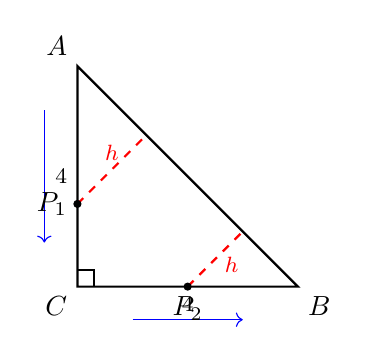
\begin{tikzpicture}[scale=0.7, thick]
  \coordinate (C) at (0,0);
  \coordinate (A) at (0,4);
  \coordinate (B) at (4,0);
  \coordinate (P1) at (0, 1.5);   % 在 AC 上，AP=2.5
  \coordinate (P2) at (2, 0);     % 在 CB 上，CP=2

  \draw (A)--(B)--(C)--cycle;

  % 直角符号
  \draw (0.3,0)--(0.3,0.3)--(0,0.3);

  % P 与 AB 的距离垂线
  % 直线 AB: x+y=4。法向 (1,1)/sqrt2
  \coordinate (H1) at ($(P1)!1!90:(A)$); % 不用计算几何，直接 foot
  % 计算 P1=(0,1.5) 到 AB 的垂足：t=((4-0-1.5)/2)=1.25 → foot=(1.25,2.75)
  \coordinate (F1) at (1.25, 2.75);
  \coordinate (F2) at (3.0, 1.0); % P2=(2,0) 到 AB: t=(4-2-0)/2=1 → foot=(3,1)
  \draw[red, dashed] (P1)--(F1);
  \draw[red, dashed] (P2)--(F2);

  \filldraw (P1) circle (1.5pt);
  \filldraw (P2) circle (1.5pt);

  % 运动方向 A→C→B
  \draw[->, blue, thin] (-0.6, 3.2) -- (-0.6, 0.8);
  \draw[->, blue, thin] (1.0, -0.6) -- (3.0, -0.6);

  \node[above left]  at (A) {$A$};
  \node[below right] at (B) {$B$};
  \node[below left]  at (C) {$C$};
  \node[left]  at (P1) {$P_1$};
  \node[below] at (P2) {$P_2$};
  \node[font=\footnotesize, red] at ($(P1)!0.5!(F1) + (0.0,0.3)$) {$h$};
  \node[font=\footnotesize, red] at ($(P2)!0.5!(F2) + (0.3,-0.1)$) {$h$};

  \node[left]  at ($(A)!0.5!(C)$) {\footnotesize $4$};
  \node[below] at ($(C)!0.5!(B)$) {\footnotesize $4$};
\end{tikzpicture}
\end{document}
